\documentclass{scrreprt}
\usepackage{listings}
\usepackage{underscore}
\usepackage{multirow}
\usepackage[utf8]{inputenc}
\usepackage{xcolor}
\usepackage{verbatim}
\usepackage{geometry} % to change the page dimensions
\geometry{a4paper} % or letterpaper (US) or a5paper or....
\setlength{\footskip}{0.3in}
\geometry{margin=1in} % for example, change the margins to 2 inches all round
\usepackage{longtable}
\usepackage{booktabs} % for much better looking tables
\usepackage{array} % for better arrays (eg matrices) in maths
\usepackage{paralist} % very flexible & customisable lists (eg. enumerate/itemize, etc.)
\usepackage{verbatim} % adds environment for commenting out blocks of text & for better verbatim
\usepackage{subfig} % make it possible to include more than one captioned figure/table in a single float
%\usepackage{graphicx} % support the \includegraphics command and options
\usepackage{graphicx}
\usepackage{color}
\usepackage{caption}
\usepackage{hyperref}
\hypersetup{
    bookmarks=true,    % show bookmarks bar?
    pdftitle={Specification},    % title
    pdfauthor={Selyunin, Pelesic, Jakovljevic},                     % author
    pdfsubject={TeX and LaTeX},                        % subject of the document
    pdfkeywords={TeX, LaTeX, graphics, images}, % list of keywords
    colorlinks=false,       % false: boxed links; true: colored links
    linkcolor=blue,       % color of internal links
    citecolor=black,       % color of links to bibliography
    filecolor=black,        % color of file links
    urlcolor=purple,        % color of external links
%    linktoc=page            % only page is linked
}
\def\myversion{1.0 }
\title{%
\flushright
\rule{16cm}{2pt}\vskip1cm
\Huge{SPECIFICATION}\\
\vspace{1cm}
%for\\
%\vspace{1cm}
Code mobility in \\Networked Embedded System\\
\vspace{1cm}
\LARGE{Release 0.0.1\\}
%\vspace{0.5cm}
%\LARGE{Version \myversion approved\\}
\vspace{1cm}
Group 4\\
\vspace{1cm}
\author{Igor Pelesi\'c, Matrikelnumber 0006828\\
Konstantin Selyunin, Matrikelnumber 1228206\\
Miljenko Jakovljevi\'c, Matrikelnumber 0426673 }
\vfill
\rule{16cm}{2pt}\vskip1cm
\date{}
\today
}
%\usepackage{etoolbox}
%\makeatletter
%\patchcmd{\chapter}{\if@openright\cleardoublepage\else\clearpage\fi}{}{}{}
%\makeatother

\makeatletter

\newcommand*{\@rowstyle}{}

\newcommand*{\rowstyle}[1]{% sets the style of the next row
  \gdef\@rowstyle{#1}%
  \@rowstyle\ignorespaces%
}

\newcolumntype{=}{% resets the row style
  >{\gdef\@rowstyle{}}%
}

\newcolumntype{+}{% adds the current row style to the next column
  >{\@rowstyle}%
}

\makeatother



\begin{document}
\maketitle
\tableofcontents

%\renewcommand{\familydefault}{\sfdefault}
\clearpage

\chapter{Introduction}

	\section{Purpose}

The specification defines the goals that should meet the project "Code mobility in Networked Embedded system". It is written by project members listed on the title page to precisely identify the goals to meet at the end of the project.
\vspace{0.1in}
\noindent
The purpose of the project is to build code mobility platform on Embedded system engineering board \cite{galler}. Our goal is to develop the system that allows users to build and execute simple agent program on top of  hardware ESE platform. To achieve the goal we propose to develop three layered structure: agent layer, platform layer, communication layer. Developer of the agent program should not aware of location of the services available on the platform and details about method to access the particular service. Given list of services agent is executed on a platform that is

	%\section{Scope}

	\section{Definitions, Acronyms, and Abbreviations}

By \emph{code mobility} we mean the capability of code to change the location where it is executed.

\vspace{0.1in}
\noindent
\emph{Strong} code mobility is the ability to allow migration of both code and execution state to the destination, \emph{weak} code mobility allows code transfer but it does not involve the transfer of the execution state.

\vspace{0.1in}
\noindent
\emph{Platform} is a component that provides corresponding hardware services to 

	\section{Background}

\noindent
The research has been done to use code mobility in distributed environment \cite{Bart1} and various application has been developed including \cite{Bart2} web application platform that allows people without major programming experience to develop the application as work-flow specification in graphical form. The use of code mobility is to "move the knowledge close to the resources" \cite{Picco} and enable higher flexibility of accessing remote resources.
	%\section{References}

	%\section{Overview}

\chapter{Requirements}	

Define requirements for the project "Code mobility in Networked Embedded system"

\renewcommand{\labelenumi}{\arabic{enumi}}
\renewcommand{\labelenumii}{\arabic{enumi}.\arabic{enumii}}

\begin{enumerate}

\item\textbf{User roles}
\begin{enumerate}

\item Application Developers (Tasks: Create control application in agent language, debug, test, prepare deployment packages)
\item Application Consumers  (Tasks: Deploy control application on target system, fill valuable bug reports)
\item Plattform Developers (Tasks: Maintenance, Extensions, Porting to another target board)
\item Maybe: Application Designers (Tasks: Design control application)
% Maybe: Application Testers (Tasks: Test control application)
\end{enumerate}


\textbf{
Global Requirements:
}


\item	\textbf{Application development requirements:}
\begin{enumerate}
\item The App Developer should be enabled to instantiate up to 4 agents on a single node, which are running concurrently.
\item The App Developer should be allowed to configure the execution scheduling of the agents via a prioriatization of the agents.
\item The platform should provide a simple agent programming language to the App Developer in which the agents of an application can be developed.
\item The agent language should provide the App Developer with the possibility to reproduce its code on another node or on another board.
\item The agent language should provide the App Developer with the possibility to communicate with another agent on the same board.
\item The agent language should provide the App Developer with the possibility to access the node hardware.
\item The agent language should provide the App Developer with the possibility to implement loops. 
\item The agent language should provide the App Developer with the possibility to compare variables.
\item The agent language should provide the App Developer with the possibility to perform addition, subtraction, multiplication and division on variables.
\item The agent language should provide the App Developer with the possibility to perform delays in the execution of code.
\item The platform should allow debugging of agents executions.
\item The platform should provide means for the creation of easily installable deployment packages.
\end{enumerate}

% The platform should provide means to add new hardware device drivers (customization).?????
%The platform should provide means to extend the agent language for own purposes (customization).????
% An Agent-Language-Assembler tool should be provided which enables the transfer of the user readable agent language to the platorm execution code,
%	which should also be easiliy extendable for customization.????

\item\textbf{Application Consumers requirements:}
\begin{enumerate}
\item The platform should provide means to deploy the agent software on the target boards easily.
\item A tracing mechanism should be provided in order to ease the process of fault detection and to allow valuable bug descriptions.
\end{enumerate}

%What do the Platform Developers need:

\item\textbf{Non-functional requirements}

\begin{enumerate}
\item The platform should be open to extensions i.e adding new hardware.
\item The agent language should be extendable.
\item Scalability
\item Documentation 
\item A platform tracing mechanism should be provided which allows for more efficient bugfixing.
\end{enumerate}


\item\textbf{What do the Application Designers need:}
\begin{enumerate}
\item A description of the platform possibilities and limitations should be provided.
\item The platform should provide means for reducing the overall complexity of a system, by allowing encapsulation of different tasks.
\item The platform should provide configurable inter agent communication facilities.
\item The platform should provide means to enable standby scenarios by allowing dynamical code reproduction.
\item The platform should provide means for strong mobility, where an agent and its execution state are transferred to a new node or board and
   the execution on the new destination is started from the memorized state.
\item A description of a platform should provide a list of all available services
\end{enumerate}

\end{enumerate}


\begin{comment}
%What do the Application Testers need:
%1) ?? To test control applications you need access to sensor data ?? Hence a test mode should be supported where sensor data are presented to the tester.

%Functional requirements

%Non-functional requirements


%Specification (based on this functional and non-functional requirements)



%User defines agents in a simple programming language (called "Agent").
%"Agents" program is interpreted on PC to bytecode.

%NES board support four platforms (nodes) for agents interactions and execution and 1 platform (node) for board-to-board communication.



%Project outline

%This will be the largest and most important section of the SRS.  The customer requirements will be embodied within Section 2, but this section will give the D-requirements that are used to guide the project’s software design, implementation, and testing.

%Each requirement in this section should be:
%•	Correct
%•	Traceable (both forward and backward to prior/future artifacts)
%•	Unambiguous
%•	Verifiable (i.e., testable)
%•	Prioritized (with respect to importance and/or stability)
%•	Complete
%•	Consistent
%•	Uniquely identifiable (usually via numbering like 3.4.5.6)

%Attention should be paid to the carefuly organize the requirements presented in this section so that they may easily accessed and understood.  Furthermore, this SRS is not the software design document, therefore one should avoid the tendency to over-constrain (and therefore design) the software project within this SRS.

	\section{External Interface Requirements}

		\subsection{User Interfaces}

		\subsection{Hardware Interfaces}

		\subsection{Software Interfaces}

		\subsection{Communications Interfaces}

	\section{Functional Requirements}
This section describes specific features of the software project.  If desired, some requirements may be specified in the use-case format and listed in the Use Cases Section.
		\subsection{Functional Requirement or Feature 1}

			\subsubsection{Introduction}

			\subsubsection{Inputs}

			\subsubsection{ Processing}

			\subsubsection{Outputs}

			\subsubsection{Error Handling}

		\subsection{ Functional Requirement or Feature 2}
…
	\section{Use Cases}

		\subsection{Use Case \#1}

		\subsection{Use Case \#2}
…
	\section{ Classes / Objects}

		\subsection{Class / Object \#1}

			\subsubsection{Attributes}

			\subsubsection{Functions}

<Reference to functional requirements and/or use cases>

		\subsection{Class / Object \#2}
…
	\section{ Non-Functional Requirements}
Non-functional requirements may exist for the following attributes.  Often these requirements must be achieved at a system-wide level rather than at a unit level.  State the requirements in the following sections in measurable terms (e.g., 95% of transaction shall be processed in less than a second, system downtime may not exceed 1 minute per day, > 30 day MTBF value, etc). 
		\subsection{Performance}

		\subsection{Reliability}

		\subsection{Availability}

		\subsection{Security}

		\subsection{Maintainability}

		\subsection{Portability}

		\section{Inverse Requirements}

State any *useful* inverse requirements.

	\section{Design Constraints}

Specify design constrains imposed by other standards, company policies, hardware limitation, etc. that will impact this software project.

	\section{Logical Database Requirements}

Will a database be used?  If so, what logical requirements exist for data formats, storage capabilities, data retention, data integrity, etc.

	\section{Other Requirements}

Catchall section for any additional requirements.

\chapter{Analysis Models}

List all analysis models used in developing specific requirements previously given in this SRS.  Each model should include an introduction and a narrative description.  Furthermore, each model should be traceable the SRS’s requirements.

	\section{Sequence Diagrams}

	\section{Data Flow Diagrams (DFD)}

	\section{State-Transition Diagrams (STD)}

\chapter{Change Management Process}

Identify and describe the process that will be used to update the SRS, as needed, when project scope or requirements change.  Who can submit changes and by what means, and how will these changes be approved.

\end{comment}

\chapter {Specification}

\section{General}

The following figure depicts the general outline of the code mobility project.

\begin{figure}[!htb]
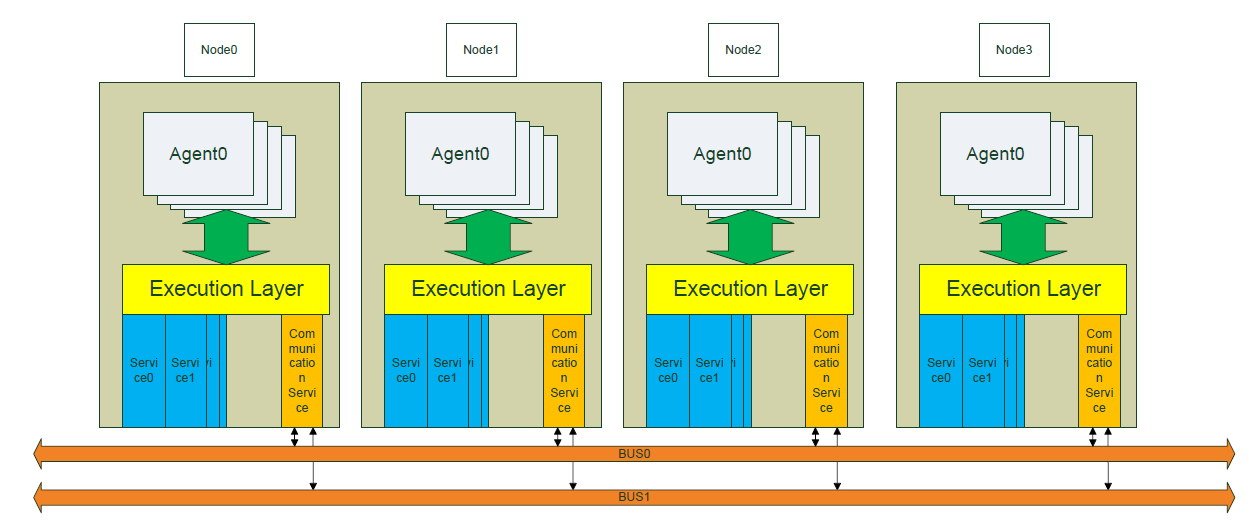
\includegraphics[scale=0.4]{figures/global.png}
\caption{Overview}
\end{figure}

On each of the 4 nodes, which can be found on the ESE board, a virtualization platform will be deployed. 
This virtualization platform will be able to execute up to 4 agents concurrently. The agents will be 
programmed in a simplistic assembler like agent language. On the platform there will be an execution 
layer which is able to execute the agent language. The agents will be able to access the hardware attached
to a node via services which are provided by the virtualization platform. Additionally the agents can
reproduce themselves to another node or even board. Within the platform a scheduler will be responsible for
providing execution time to each of the agents according to their priority. 

\section{Virtualization Platform}
The main task of the virtualization platform is to interprete the agent language commands of the agents 
and to provide them access to the hardware attached to a node via well defined interfaces. Additionally 
the platform should allow the concurrent execution of the agents. Therefore some basic means for code and 
data protection for the agent memory is required. This is achieved by assigning each of the agents an own 
memory segment and not allowing any other agent to access any other memory but its own. If some collaboration 
between the agents is required this must be requested via the communication service. The metadata of an agent 
as its code and memory segment will be stored in a structure that is shown in the figure below. 


\begin{figure}[!htbp]
\begin{center}
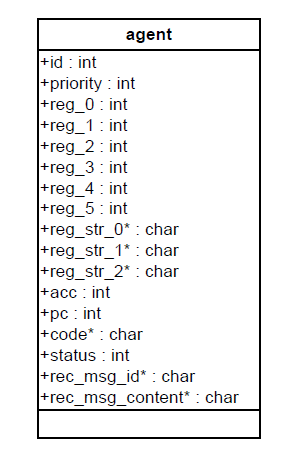
\includegraphics[scale=0.4]{figures/agent.png}
\caption{Agent structure}
\end{center}
\label{agent}
\end{figure}

Every agent has a unique id within the virtualization platform. Additionally a priority and a status for the
scheduler are stored. Assigning these values for an agent lies within the scope of an agent developer. 
Reproducing an agent on a virtualization platform where the agent’s id is already used will result in a denial 
of the reproduction by the platform. Every agent has 6 numerical general purpose registers used for the execution
of the agent language. Additonally there are 3 char general purpose registers. The result of every agent language 
command will be written to the accumulator. There is also a program counter which is used for the execution of the
agent and the numerical agent language representation is stored as well. The agent structure also contains a buffer
for receiving messages from other agents and variable to store the id of the received message.


\noindent
In order to reproduce the agent on another board or node the agent’s structure needs to be serialized and transmitted via the communication layer.


\noindent
Additionally the virtualization platform has to provide the agent developer with some means to deploy the agent
executable to the virtualization platform, during compilation of the platform. During the initialization of the
platform all deployed agents should be instantiated on the given platform.

\section{Execution Layer}

The execution layer is responsible for the execution of an agent which is written in the agent language and later translated to agent opcodes. 
The agent language provides means for:
\begin{itemize}
 \item storing values to the general purpose registers
 \item comparing the contents of the general purpose registers 
 \item performing basic mathematical functions like addition, subtraction, multiplication and division
 \item a jump operation 
 \item reproduction and cloning functions
 \item sleep, delay and terminate functions
 \item functions to access the hardware attached to a node
\end{itemize}


\noindent
If a function of the agent language returns a value, this value will be stored in the accumulator, 
where it can be used later on for further operations e.g. comparison etc. 


\noindent
The basic workflow of the execution layer as soon it is called by the scheduler is to read the next 
agent language opcode (all agent opcodes have a fixed length) as identified by the program counter, 
to decode it and to perform the function which is described by the opcode. Eventually the program 
counter value is changed and the control is returned back to the scheduler. 

\begin{figure}[!htbp]
\begin{center}
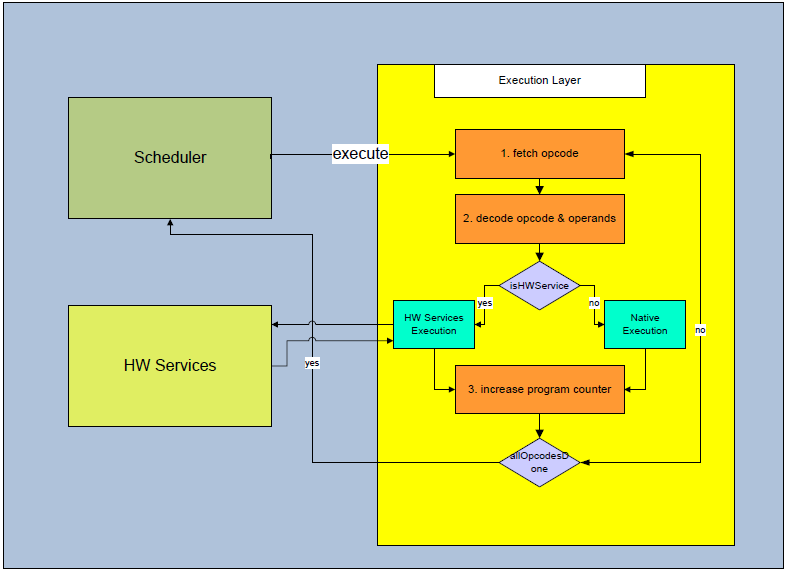
\includegraphics[scale=0.4]{figures/exelayer.png}
\caption{Execution Layer}
\end{center}
\label{exelayer}
\end{figure}



The execution layer is 
called by the method execute which takes the following input parameters:
\begin{itemize}
 \item Pointer to a specific agent structure
 \item Number of opcodes to execute
\end{itemize}

\begin{figure}[!htb]
\lstset{language=C}
\begin{lstlisting}[frame=single]
/**
	Function : execute
		excutes the next opcodes of an agent
	Returns : 
		the amount of successfully executed opcoded
	Parameters : 
		agent : agent status structure
		opcode: amount of opcodes to be executed
**/
uint8_t execute(agent_t* agent, uint8_t opcode)
\end{lstlisting}
\caption{Executing agent language opcode}
\label{fig:excopc}
\end{figure}



\section{Hardware Services}

The virtualization platform provides access to the hardware attached to a node via according hardware 
device drivers. The methods of the device drivers are made public to the execution layer which in turns 
allows the agents to access these methods. As the hardware supported by a node differs from node to node 
the virtualization platform should be able to discover during its initialization which hardware is supported 
on the node where it’s running. 


\noindent
This will be achieved by defining a global set of function pointers within the virtualization platform. 
This set should contain all possible methods of all available device drivers. During initialization the platform 
will assign the according function pointer to a method provided by the device driver if the device is supported, 
otherwise the according function pointer will stay null. 

\begin{figure}[!htb]
\lstset{language=C}
\begin{lstlisting}[frame=single]
typedef struct {

	void (*init_bargraph)(void);
	void (*set_bargraph)(uint8_t value);

	void (*clk_init)(void);
	uint32_t (*clk_get_time)(void);

	void (*init_cooler)(void);
	void (*set_cooler)(uint8_t duty_cycle);

	void (*DISPLAY_init)(void);
	void (*DISPLAY_drawBg)(uint16_t rgb);
	uint8_t (*DISPLAY_drawElement)(uint8_t row, uint8_t col,
		uint16_t rgb, DisplayObject_t object);
	
	void (*DISPLAY_drawBorder)(void);
	
	uint8_t (*DISPLAY_drawPoints)(uint8_t player_id, 
		uint8_t points);

	void (*heater_init)(void);
	void (*heater_set)(uint8_t duty_cycle);

	void (*init_pushbutton0)(void (*callback)(void));
	void (*init_pushbutton1)(void (*callback)(void));

	void (*therm_init)(void);
	int16_t (*therm_get_temp)(uint8_t name);

} drivers_t;
\end{lstlisting}
\caption{Device drivers methods}
\label{fig:devicedrivers}
\end{figure}

\noindent
All device drivers should support init methods, which will be called by the platform during its initialization. 
Even if a hardware device is not supported on a given node, there should be at least a dummy device driver for it present, 
providing an empty init method. A real device driver should register its methods to the global function pointers during its 
init_driver method execution. Choosing this approach we would reach some form of modularity which would allow us to exchange 
to device drivers without necessity to change the platform code.

\noindent
If an interaction with a device driver is blocking, then the calling agent will be put to status blocking unless there is an answer from
the device driver.

\section{Communication Layer}

The agents should be able to communicate with other agents on the same node or on the same board. Therefore the agent 
language provides means to request the sending or receiving of a message.  


\noindent
The sending function is blocking the further execution of the agent until the message is sent respectively received. 
When an agent wants to send a message this message is proceeded to the communications service which takes care of the 
actual transmission. While the sending procedure is ongoing the further execution of the sending agent is blocked. 
Its status in the agent structure is set to “blocked”. As soon as the communication service signalizes a successful 
message transmission or a failure the result of the sending function is written to the accumulator and the agent will 
be made available for further execution.  


\noindent
When an agent sends a message to another agent, the receiving platform stores the id of the message and its content 
to the receiver agent structure. The receiving agent is able to retrieve the last message from its buffer. 
However only one message can be stored within the receiving agent structure and the next message will overwrite the 
content and possible the id of the last message.  


\noindent
The communication service provides no guarantees that sending of a message will succeed; it works on a best effort 
approach. Therefore the agent developer has to make sure by reading the return value of a sending operation whether 
the message was successfully sent or not and should initialize a retransmission in case of failure. 


\noindent
Every message sent should be identified by an id, in order to allow the transmission of messages with different semantics.

The receiver of a message should be identified via the node number (0..3) where the receiving agent is currently expected
 to be running and the receiver agent id. As the ids of agents are within the scope of the agent developer she has to make 
sure, that the correct receiving agent is addressed.Additionally a multicast message could be supported by allowing omitting 
the node address which should result in sending the message to all agents identified by the provided id. 

\section{Scheduler}
The main task of the scheduler which is part of the virtualization platform is to identify the next agent to be executed 
and to utilize the execution layer to perform the execution of the according agent. The decision which agent to be chosen 
should be made on a static priority based scheduling policy.


\noindent
Every agent is assigned a priority (0..3) by the agent developer which is stored within the agent structure. 
The highest priority is 3 and the lowest priority is 0. Based on the priorities of the currently running agents 
the scheduler creates a static list by which the order of the agent execution is defined. The scheduler instructs 
the execution layer to execute exactly priority + 1 opcodes for a given agent. Eventually the control returns to 
the scheduler and the next agent from the list is picked. The list is iterated cyclically.

\begin{figure}[!htbp]
\begin{center}
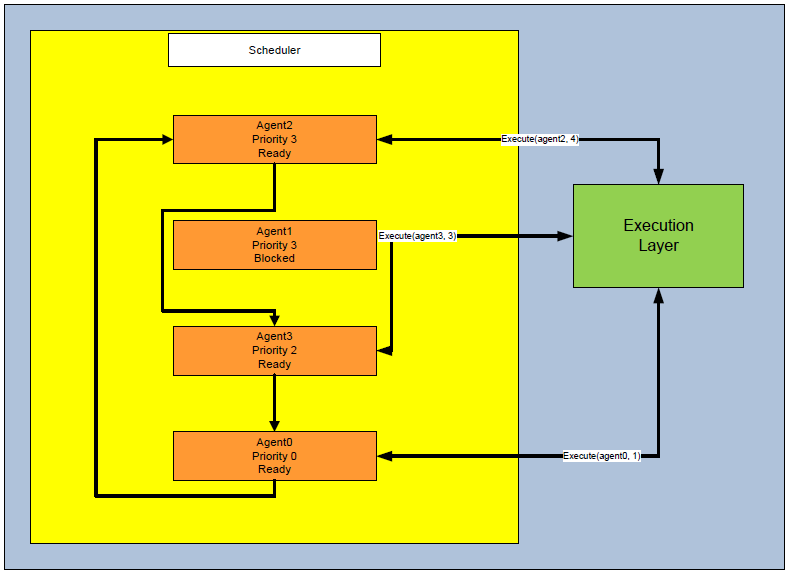
\includegraphics[scale=0.4]{figures/scheduler.png}
\caption{Scheduler}
\end{center}
\label{scheduler}
\end{figure}


\noindent
If an agent which is to be scheduled next is currently blocked by a sending operation, then its execution should be omitted. 


\noindent
As an agent can reproduce it self to another node or board or clone itself within the same platform the scheduling 
list requires adaptation as soon as new agent is deployed on a platform. Whenever a given platform is the destination 
end point of a reproduction respectively cloning operation the scheduler needs to update its scheduling list before proceeding with further executions.

\section{Agent language}

\subsection{Agent language (Assembler level)}
\noindent
To develop a mobile agent \textit{Agent language} will be used. Language is tied to agent internal structure and support necessary operation for code mobility and message exchange. While writing the program for agent user should not be aware of hardware services presented on a given platform, but have common knowledge about all available services and what operations are allowed to do with the services (have list of services and available operations). It is the responsibility of the platform to provide required service to the agent (perform measurement, IO operation) or to manifest an error if the service is not available on the given platform. All current variables are allowed to store only in registers of agent structure (Fig. ~\ref{agent}).


\noindent
The language supports the following groups of operations: arithmetic, control flow, code mobility, message exchange , access to hardware services.


\begin{tabular}{|l|c|l|c|}
\hline
\multicolumn{4}{|c|}{\textbf{Addressing registers of agent structure}}\\
\hline
\multicolumn{2}{|c|}{\textbf{General purpose registers}} & \multicolumn{2}{c|}{\textbf{Character registers}}\\
\hline
Register & \texttt{rrrr} & Char Register & \texttt{rrrr}\\
\hline
\texttt{reg_0} & \texttt{0000} & \texttt{reg_str_0} & \texttt{1000}\\
\hline
\texttt{reg_1} & \texttt{0001} & \texttt{reg_str_1} & \texttt{1001}\\
\hline
\texttt{reg_2} & \texttt{0010} & \texttt{reg_str_2} & \texttt{1010}\\
\hline
\texttt{reg_3} & \texttt{0011} &   &  \\
\hline
\texttt{reg_4} & \texttt{0100} &   &  \\
\hline
\texttt{reg_5} & \texttt{0101} &   &  \\
\hline
\texttt{reg_6} & \texttt{0110} &   &  \\
\hline
%\texttt{reg_7} & \texttt{0111} &   &  \\
%\hline
\end{tabular}

\subsubsection{Arithmetic operations of agent assembly language}
\noindent
\textbf{Addition}

\noindent
Add the content of \texttt{reg_d} and \texttt{reg_r} (or \texttt{value}) and put the result into \texttt{acc}.\\
\noindent
\framebox{\texttt{add reg_d, reg_r}}

\noindent
\begin{tabular}{+p{1.3in}+p{2.2in}+p{1.3in}+p{1in}}

Syntax  & Operands   & Program counter & Flags\\

\texttt{add reg_d, reg_r} & \texttt{reg_0 $\leq$ reg_d $\leq$ reg_6, reg_0 $\leq$ reg_r $\leq$ reg_6} & \texttt{PC = PC + 1} & \texttt{C} \\

\multicolumn{2}{l}{Operation} & & \\

\multicolumn{2}{l}{\texttt{acc $\leftarrow$ reg_d + reg_r}} & & \\

\end{tabular}

\noindent
16-bit opcode:

\noindent
\begin{tabular}{|c|c|c|c|}
\multicolumn{2}{|l|}{} & reg_d & reg_r\\
\hline
\texttt{0000} & \texttt{0011} & \texttt{dddd} & \texttt{rrrr}\\

\end{tabular}

\vspace{0.5in}
\noindent
\framebox{\texttt{add reg_r, value}}
\vspace{0.2in}

\noindent
\begin{tabular}{+p{1.3in}+p{2.2in}+p{1.3in}+p{1in}}

Syntax  & Operands   & Program counter & Flags\\

\texttt{add reg_r, value} & \texttt{reg_0 $\leq$ reg_r $\leq$ reg_6, 0x00 $\leq$ value $\leq$ 0xFF} & \texttt{PC = PC + 1} & \texttt{C} \\

\multicolumn{2}{l}{Operation} & & \\

\multicolumn{2}{l}{\texttt{acc $\leftarrow$ reg_r + value}} & & \\

\end{tabular}

\noindent
16-bit opcode:

\noindent
\begin{tabular}{|c|c|c|c|}
 & reg_r & \multicolumn{2}{c|}{value}\\
\hline
\texttt{0011} & \texttt{rrrr} & \texttt{vvvv} & \texttt{vvvv}\\

\end{tabular}

\vspace{0.5in}

\noindent
\textbf{Subtraction}

\noindent
Subtract \texttt{reg_s} (or \texttt{value}) from \texttt{reg_m} and put the result into \texttt{acc}.\\
\noindent
\framebox{\texttt{sub reg_m, reg_s}}

\noindent
\begin{tabular}{+p{1.3in}+p{2.2in}+p{1.3in}+p{1in}}

Syntax  & Operands   & Program counter & Flags\\

\texttt{sub reg_m, reg_s} & \texttt{reg_0 $\leq$ reg_m $\leq$ reg_6, reg_0 $\leq$ reg_s $\leq$ reg_6} & \texttt{PC = PC + 1} & \texttt{C} \\

\multicolumn{2}{l}{Operation} & & \\

\multicolumn{2}{l}{\texttt{acc $\leftarrow$ reg_m - reg_s}} & & \\

\end{tabular}

\noindent
16-bit opcode:

\noindent
\begin{tabular}{|c|c|c|c|}
\multicolumn{2}{|l|}{} & reg_m & reg_s\\
\hline
\texttt{0000} & \texttt{0110} & \texttt{mmmm} & \texttt{ssss}\\

\end{tabular}

\vspace{0.5in}
\noindent
\framebox{\texttt{sub reg_m, value}}
\vspace{0.1in}

\noindent
\begin{tabular}{+p{1.3in}+p{2.2in}+p{1.3in}+p{1in}}

Syntax  & Operands   & Program counter & Flags\\

\texttt{sub reg_m, value} & \texttt{reg_0 $\leq$ reg_m $\leq$ reg_6, 0x00 $\leq$ value $\leq$ 0xFF} & \texttt{PC = PC + 1} & \texttt{C} \\

\multicolumn{2}{l}{Operation} & & \\

\multicolumn{2}{l}{\texttt{acc $\leftarrow$ reg_m - value}} & & \\

\end{tabular}

\noindent
16-bit opcode:

\noindent
\begin{tabular}{|c|c|c|c|}
 & reg_m & \multicolumn{2}{c|}{value}\\
\hline
\texttt{0110} & \texttt{mmmm} & \texttt{vvvv} & \texttt{vvvv}\\

\end{tabular}

\vspace{0.5in}



\noindent
\textbf{Division}

\noindent
Divide reg1 by reg2 (or value) and put the result into acc.\\
\noindent
\framebox{\texttt{div reg_d, reg_r}}

\noindent
\begin{tabular}{+p{1.3in}+p{2.2in}+p{1.3in}+p{1in}}

Syntax  & Operands   & Program counter & Flags\\

\texttt{div reg_d, reg_r} & \texttt{reg_0 $\leq$ reg_d $\leq$ reg_6, reg_0 $\leq$ reg_r $\leq$ reg_6} & \texttt{PC = PC + 1} & \texttt{C} \\

\multicolumn{2}{l}{Operation} & & \\

\multicolumn{2}{l}{\texttt{acc $\leftarrow$ reg_d / reg_r}} & & \\

\end{tabular}

\noindent
16-bit opcode:

\noindent
\begin{tabular}{|c|c|c|c|}
\multicolumn{2}{|l|}{} & reg_d & reg_r\\
\hline
\texttt{0000} & \texttt{1001} & \texttt{dddd} & \texttt{rrrr}\\

\end{tabular}

\vspace{0.5in}
\noindent
\framebox{\texttt{div reg_d, value}}
\vspace{0.1in}

\noindent
\begin{tabular}{+p{1.3in}+p{2.2in}+p{1.3in}+p{1in}}

Syntax  		  & Operands   								     & Program counter       & Flags\\

\texttt{div reg_d, value} & \texttt{reg_0 $\leq$ reg_d $\leq$ reg_6, 0x00 $\leq$ value $\leq$ 0xFF} & \texttt{PC = PC + 1} & \texttt{C} \\

\multicolumn{2}{l}{Operation} 									      & 		     & \\

\multicolumn{2}{l}{\texttt{acc $\leftarrow$ reg_d / value}} & & \\

\end{tabular}

\noindent
16-bit opcode:

\noindent
\begin{tabular}{|c|c|c|c|}
 & reg_d & \multicolumn{2}{c|}{value}\\
\hline
\texttt{1001} & \texttt{dddd} & \texttt{vvvv} & \texttt{vvvv}\\

\end{tabular}

\vspace{0.2in}

\noindent
\textbf{Multiplication}


\noindent
Multiply \texttt{reg1} and \texttt{reg2} (or \texttt{value}) and put the result into \texttt{acc}.\\
\noindent
\framebox{\texttt{mul reg_d, reg_r}}

\noindent
\begin{tabular}{+p{1.3in}+p{2.2in}+p{1.3in}+p{1in}}

Syntax  & Operands   & Program counter & Flags\\

\texttt{mul reg_d, reg_r} & \texttt{reg_0 $\leq$ reg_d $\leq$ reg_6, reg_0 $\leq$ reg_r $\leq$ reg_6} & \texttt{PC = PC + 1} & \texttt{C} \\

\multicolumn{2}{l}{Operation} & & \\

\multicolumn{2}{l}{\texttt{acc $\leftarrow$ reg_d * reg_r}} & & \\

\end{tabular}

\noindent
16-bit opcode:

\noindent
\begin{tabular}{|c|c|c|c|}
\multicolumn{2}{|l|}{} & reg_d & reg_r\\
\hline
\texttt{0000} & \texttt{1100} & \texttt{dddd} & \texttt{rrrr}\\

\end{tabular}

\vspace{0.5in}
\noindent
\framebox{\texttt{mul reg1, value}}
\vspace{0.1in}

\noindent
\begin{tabular}{+p{1.3in}+p{2.2in}+p{1.3in}+p{1in}}

Syntax  		  & Operands   								     & Program counter       & Flags\\

\texttt{mul reg_d, value} & \texttt{reg_0 $\leq$ reg_d $\leq$ reg_6, 0x00 $\leq$ value $\leq$ 0xFF} & \texttt{PC = PC + 1} & \texttt{C} \\

\multicolumn{2}{l}{Operation} 									      & 		     & \\

\multicolumn{2}{l}{\texttt{acc $\leftarrow$ reg_d * value}} & & \\

\end{tabular}

\noindent
16-bit opcode:

\noindent
\begin{tabular}{|c|c|c|c|}
 & reg_d & \multicolumn{2}{c|}{value}\\
\hline
\texttt{1100} & \texttt{dddd} & \texttt{vvvv} & \texttt{vvvv}\\

\end{tabular}


\subsubsection{Control flow operations and comparison in agent assembly language}
\noindent
\textbf{Jump if greater}

\noindent
Jump to  \texttt{offset} in code segment of agent structure if the value of \texttt{acc}. is 1.

\noindent
\framebox{\texttt{jmpgr  offset}}
\vspace{0.1in}

\noindent
\begin{tabular}{+p{1.3in}+p{2.2in}+p{2.3in}}
Syntax  		  & Operands   								     & Program counter       \\

\texttt{jmpgr  offset} & \texttt{-128 $\leq$ offset $\leq$ +127} & \texttt{PC = PC + offset +1} if \texttt{acc = 1}, \texttt{PC = PC + 1} otherwise \\

\end{tabular}

\noindent
16-bit opcode:

\noindent
\begin{tabular}{|c|c|c|c|}
 \multicolumn{2}{|c|}{} & \multicolumn{2}{c|}{offset}\\
\hline
\texttt{1111} & \texttt{0011} & \texttt{vvvv} & \texttt{vvvv}\\

\end{tabular}

\vspace{0.4in}
\noindent
\textbf{Jump if equal}

\noindent
Jump to \texttt{offset} in code segment of agent structure if the value of acc. is 0.

\noindent
\framebox{\texttt{jmpeq  offset}}
\vspace{0.1in}

\noindent
\begin{tabular}{+p{1.3in}+p{2.2in}+p{2.3in}}
Syntax  		  & Operands   								     & Program counter       \\

\texttt{jmpeq  offset} & \texttt{-128 $\leq$ offset $\leq$ +127} & \texttt{PC = PC + offset +1} if \texttt{acc = 0}, \texttt{PC = PC + 1} otherwise \\

\end{tabular}

\noindent
16-bit opcode:

\noindent
\begin{tabular}{|c|c|c|c|}
 \multicolumn{2}{|c|}{} & \multicolumn{2}{c|}{offset}\\
\hline
\texttt{1111} & \texttt{0110} & \texttt{vvvv} & \texttt{vvvv}\\

\end{tabular}


\vspace{0.4in}
\noindent
\textbf{Jump if less}

\noindent
Jump to \texttt{offset} in code segment of agent structure if the value of acc. is -1.

\noindent
\framebox{\texttt{jmpls  offset}}
\vspace{0.1in}

\noindent
\begin{tabular}{+p{1.3in}+p{2.2in}+p{2.4in}}
Syntax  		  & Operands   								     & Program counter       \\

\texttt{jmpls  offset} & \texttt{-128 $\leq$ offset $\leq$ +127} & \texttt{PC = PC + offset +1} if \texttt{acc = -1}, \texttt{PC = PC + 1} otherwise \\

\end{tabular}

\noindent
16-bit opcode:

\noindent
\begin{tabular}{|c|c|c|c|}
 \multicolumn{2}{|c|}{} & \multicolumn{2}{c|}{offset}\\
\hline
\texttt{1111} & \texttt{1100} & \texttt{vvvv} & \texttt{vvvv}\\

\end{tabular}

\vspace{0.4in}
\noindent
\textbf{Comparison}

\noindent
Compare \texttt{reg1} and \texttt{reg2} (or \texttt{value}).

%\noindent
%If reg1 $>$ reg2 put 1 into acc,

%\noindent
%if reg1 $=$ reg2 put 0 into acc,

%\noindent
%if reg1 $<$ reg2 put -1 into acc.

\noindent
\framebox{\texttt{compare reg_d, reg_r}}

\noindent
\begin{tabular}{+p{1.8in}+p{2.2in}+p{1.3in}}

Syntax  & Operands   & Program counter \\

\texttt{compare reg_d, reg_r} & \texttt{reg_0 $\leq$ reg_d $\leq$ reg_6, reg_0 $\leq$ reg_r $\leq$ reg_6} & \texttt{PC = PC + 1} \\

\multicolumn{3}{l}{Operation} \\

\multicolumn{2}{l}{\texttt{acc $\leftarrow$ 1} if (reg_d - reg_r $>$ 0)}  & \\
\multicolumn{2}{l}{\texttt{acc $\leftarrow$ 0} if (reg_d - reg_r $=$ 0)}  & \\
\multicolumn{2}{l}{\texttt{acc $\leftarrow$ -1} if (reg_d - reg_r $<$ 0)}  & \\
\end{tabular}

\noindent
16-bit opcode:

\noindent
\begin{tabular}{|c|c|c|c|}
\multicolumn{2}{|l|}{} & reg_d & reg_r\\
\hline
\texttt{0000} & \texttt{1010} & \texttt{dddd} & \texttt{rrrr}\\

\end{tabular}

\vspace{0.4in}
\noindent
\framebox{\texttt{compare reg_d, value}}

\noindent
\begin{tabular}{+p{1.9in}+p{2.2in}+p{1.3in}}

Syntax  & Operands   & Program counter \\

\texttt{compare reg_d, value} & \texttt{reg_0 $\leq$ reg_d $\leq$ reg_6, 0x00 $\leq$ value $\leq$ 0xFF} & \texttt{PC = PC + 1} \\

\multicolumn{3}{l}{Operation} \\

\multicolumn{2}{l}{\texttt{acc $\leftarrow$ 1} if (reg_d - value $>$ 0)}  & \\
\multicolumn{2}{l}{\texttt{acc $\leftarrow$ 0} if (reg_d - value $=$ 0)}  & \\
\multicolumn{2}{l}{\texttt{acc $\leftarrow$ -1} if (reg_d - value $<$ 0)}  & \\
\end{tabular}

\noindent
16-bit opcode:

\noindent
\begin{tabular}{|c|c|c|c|}
 & reg_r & \multicolumn{2}{c|}{value}\\
\hline
\texttt{1010} & \texttt{rrrr} & \texttt{vvvv} & \texttt{vvvv}\\

\end{tabular}

\vspace{0.5in}

\subsubsection{Code mobility operations of agent assembly language}
\noindent
\textbf{Move code}

\noindent
Move agent structure to platform that possess required service

\noindent
\framebox{\texttt{move service}}
\vspace{0.1in}

\begin{tabular}{+p{1.3in}+p{2.8in}+p{1.3in}}

Syntax  & Operands   & Program counter \\

\texttt{move service} & \texttt{service_0 $\leq$ service $\leq$ service_10} & \texttt{PC = PC + 1} \\

\multicolumn{3}{l}{Operation} \\

\multicolumn{3}{l}{Serialize and transmit agent structure to the platform that possess required service}  \\

\end{tabular}

\vspace{0.1in}
\noindent
16-bit opcode:

\noindent
\begin{tabular}{|c|c|c|c|}
 & reg_r & \multicolumn{2}{c|}{service}\\
\hline
\texttt{1111} & \texttt{0001} & \texttt{ssss} & \texttt{ssss}\\

\end{tabular}

\vspace{0.5in}
\noindent
\textbf{Clone code}

\noindent
Replicate agent structure on the given platform

\noindent
\framebox{\texttt{clone}}
\vspace{0.1in}

\begin{tabular}{+p{1.3in}+p{1.3in}}

Syntax    & Program counter \\

\texttt{clone}  & \texttt{PC = PC + 1} \\

\end{tabular}

\vspace{0.1in}
\noindent
16-bit opcode:

\noindent
\begin{tabular}{|c|c|c|c|}
  \multicolumn{4}{|c|}{}\\
\hline
\texttt{1111} & \texttt{0010} & \texttt{0000} & \texttt{0000}\\

\end{tabular}

\vspace{0.4in}
\noindent
\textbf{Die}

\noindent
Destroy agent structure and free corresponding memory

\noindent
\framebox{\texttt{die}}

\vspace{0.1in}
\noindent
16-bit opcode:

\noindent
\begin{tabular}{|c|c|c|c|}
  \multicolumn{4}{|c|}{}\\
\hline
\texttt{1111} & \texttt{0100} & \texttt{0000} & \texttt{0000}\\
\end{tabular}

\subsubsection{Message exchange}
\noindent
\textbf{Send}

\noindent
Send message of predefined \texttt{type} to \texttt{platform}.

\noindent
\framebox{\texttt{sendmsg type, platform}}
\vspace{0.1in}


\noindent
\begin{tabular}{+p{1.9in}+p{2.5in}+p{1.3in}}

Syntax  & Operands   & Program counter \\

\texttt{sendmsg platform} & \texttt{platform_0 $\leq$ platform $\leq$ platform_3} & \texttt{PC = PC + 1}\\
\multicolumn{3}{l}{Operation} \\
\multicolumn{3}{l}{Send \texttt{mess_type} to \texttt{platform}} \\

\end{tabular}

\noindent
16-bit opcode:

\noindent
\begin{tabular}{|c|c|c|c|}
 \multicolumn{2}{|c|}{} & type & platform\\
\hline
\texttt{1111} & \texttt{1000} & \texttt{tttt} & \texttt{pppp}\\

\end{tabular}


\vspace{0.5in}
\noindent
\textbf{Receive}

\noindent
Pull message from \texttt{platform} to acc.

\noindent
\framebox{\texttt{pullmsg}}

\noindent
\begin{tabular}{+p{1.9in}+p{1.3in}}

Syntax   & Program counter \\

\texttt{pullmsg}  & \texttt{PC = PC + 1} \\

\multicolumn{2}{l}{Operation} \\

\multicolumn{2}{l}{ \texttt{acc $\leftarrow$} msg_type, msg_platform} \\

\end{tabular}

\noindent
16-bit opcode:

\noindent
\begin{tabular}{|c|c|c|c|}
 \multicolumn{4}{|c|}{} \\
\hline
\texttt{1111} & \texttt{1010} & \texttt{0000} & \texttt{0000}\\
\end{tabular}

\vspace{0.1in}
\subsubsection{Store, move and wait operations}
\noindent
\textbf{Store}

\noindent
Store value in register

\noindent
Store character in register

\noindent
\framebox{\texttt{store reg_d, value}}

\noindent
\begin{tabular}{+p{1.8in}+p{2.2in}+p{1.3in}}

Syntax  		  & Operands   								     & Program counter       \\

\texttt{store reg_d, value} & \texttt{reg_0 $\leq$ reg_d $\leq$ reg_6, 0x00 $\leq$ value $\leq$ 0xFF} & \texttt{PC = PC + 1}  \\

\multicolumn{2}{l}{Operation} 									      & 		     \\

\multicolumn{2}{l}{\texttt{reg_d $\leftarrow$ value}} & \\

\end{tabular}

\noindent
16-bit opcode:

\noindent
\begin{tabular}{|c|c|c|c|}
 & reg_d & \multicolumn{2}{c|}{value}\\
\hline
\texttt{1101} & \texttt{dddd} & \texttt{vvvv} & \texttt{vvvv}\\

\end{tabular}

\vspace{0.4in}
\noindent
\framebox{\texttt{storecr reg_str, char}}
\vspace{0.1in}

\noindent
\begin{tabular}{+p{1.8in}+p{2.2in}+p{1.3in}}

Syntax  		  & Operands   						    & Program counter       \\

\texttt{storecr reg_str, char} & \texttt{reg_str_0 $\leq$ reg_str $\leq$ reg_str_2} & \texttt{PC = PC + 1}  \\

\multicolumn{2}{l}{Operation} 									      & 		     \\

\multicolumn{2}{l}{\texttt{reg_str $\leftarrow$ value}} & \\

\end{tabular}

\noindent
16-bit opcode:

\noindent
\begin{tabular}{|c|c|c|c|}
 & reg_str & \multicolumn{2}{c|}{value}\\
\hline
\texttt{1011} & \texttt{rrrr} & \texttt{vvvv} & \texttt{vvvv}\\

\end{tabular}

\vspace{0.4in}
\noindent
\textbf{Move}

\noindent
Move value from reg_r to reg_d

\noindent
\framebox{\texttt{mv reg_d, reg_r}}

\noindent
\begin{tabular}{+p{1.8in}+p{2.2in}+p{1.3in}}

Syntax  		  & Operands   								     & Program counter       \\

\texttt{mv reg_d, reg_r} & \texttt{reg_0 $\leq$ reg_d $\leq$ reg_6, reg_0 $\leq$ reg_r $\leq$ reg_6} & \texttt{PC = PC + 1}  \\

\multicolumn{2}{l}{Operation} 									      & 		     \\

\multicolumn{2}{l}{\texttt{reg_d $\leftarrow$ reg_r}} & \\

\end{tabular}

\noindent
16-bit opcode:

\noindent
\begin{tabular}{|c|c|c|c|}
 \multicolumn{2}{|c|}{value} & reg_d & reg_r\\
\hline
\texttt{0000} & \texttt{1101} & \texttt{dddd} & \texttt{rrrr}\\

\end{tabular}

\vspace{0.5in}

\noindent
\textbf{Wait}

\noindent
Wait for ms


\noindent
\framebox{\texttt{wait delay_ms}}

\noindent
\begin{tabular}{+p{1.8in}+p{2.2in}+p{1.3in}}

Syntax  		  & Operands   								     & Program counter       \\

\texttt{wait delay_ms} & \texttt{0 $\leq$ delay_ms $\leq$ 0xFF} & \texttt{PC = PC + 1}  \\


\end{tabular}

\noindent
16-bit opcode:

\noindent
\begin{tabular}{|c|c|c|c|}
 \multicolumn{2}{|c|}{} & \multicolumn{2}{c|}{delay}\\
\hline
\texttt{0000} & \texttt{0101} & \texttt{dddd} & \texttt{dddd}\\

\end{tabular}
\vspace{0.4in}

\noindent
\textbf{Assign priority value}


\noindent
Assign priority of the agent to value in range 0..3

\noindent
\framebox{\texttt{priority value}}


\noindent
\begin{tabular}{+p{1.8in}+p{2.2in}+p{1.3in}}

Syntax  		  & Operands   								     & Program counter       \\

\texttt{priority value} & \texttt{0 $\leq$ value $\leq$ 3} & \texttt{PC = PC + 1}  \\

\multicolumn{2}{l}{Operation} 									      & 		     \\

\multicolumn{2}{l}{\texttt{priority $\leftarrow$ value}} & \\

\end{tabular}

\noindent
16-bit opcode:

\noindent
\begin{tabular}{|c|c|c|c|}
 \multicolumn{2}{|c|}{} &  \multicolumn{2}{c|}{priority}\\
\hline
\texttt{0000} & \texttt{1000} & \texttt{pppp} & \texttt{pppp}\\

\end{tabular}

\vspace{0.4in}
\subsubsection{Access to hardware services}
\noindent
\textbf{Set}

\noindent
Set service to reg or value

\noindent
\framebox{\texttt{setservice service, reg}}

\noindent
\begin{tabular}{+p{1.9in}+p{2.9in}+p{1.2in}}

Syntax  		  & Operands   								     & Program counter       \\

\texttt{setservice service, reg} & \texttt{service_0 $\leq$ service $\leq$ service_10, reg_0 $\leq$ reg $\leq$ reg_6} & \texttt{PC = PC + 1}  \\

\end{tabular}

\noindent
16-bit opcode:

\noindent
\begin{tabular}{|c|c|c|c|}
 & reg & \multicolumn{2}{c|}{service}\\
\hline
\texttt{0111} & \texttt{rrrr} & \texttt{ssss} & \texttt{ssss}\\

\end{tabular}
\vspace{0.1in}
%\noindent
%\framebox{\texttt{setservice value}}
%\vspace{0.1in}

\noindent
\textbf{Get}

\noindent
Put corresponding value from the service to the acc.

\noindent
\framebox{\texttt{getservice}}
\vspace{0.1in}

\noindent
\begin{tabular}{+p{1.9in}+p{1.2in}}

Syntax  		 & Program counter       \\

\texttt{getservice} & \texttt{PC = PC + 1}  \\

\end{tabular}

\noindent
16-bit opcode:

\noindent
\begin{tabular}{|c|c|c|c|}
 \multicolumn{4}{|c|}{}\\
\hline
\texttt{0000} & \texttt{0111} & \texttt{0000} & \texttt{0000}\\

\end{tabular}
\vspace{0.1in}

\begin{comment}
, comparison of operands, jump and loop constructs, as well as operations related to code mobility ( move to service, clone, die). Developer of agent program should not be aware of present services on the 
The agent developer use the following language to develop the program.
Program consist of single possible recursive function. The language has two types: integer and string.


\begin{longtable}{|l|p{5in}|}
\hline
Lexical elements	
&
Agent program includes the following lexical elements
\\
\hline
keyword
&
'function' $~\mid~$ 'var' $~\mid~$ 'int' $~\mid~$ 'char' $~\mid~$ 'boolean' $~\mid~$ 'true' $~\mid~$ 'false' $~\mid~$ 'this' $~\mid~$ 'if' $~\mid~$ 'else' $~\mid~$ 'while' $~\mid~$ 'return' $~\mid~$ 'move' $~\mid~$ 'clone' $~\mid~$  'message' $~\mid~$  'to'  $~\mid~$  
\\
\hline
symbol
&
$~\mid~$  '\{'  $~\mid~$  '\}'  $~\mid~$  '('  $~\mid~$  ')'  $~\mid~$  '['  $~\mid~$  ']'  $~\mid~$  '.'  $~\mid~$  ','  $~\mid~$  ';'  $~\mid~$  '+'  $~\mid~$  '-'  $~\mid~$  '*'  $~\mid~$  '/'  $~\mid~$  '\&'  $~\mid~$  '$~\mid~$'  $~\mid~$  '<'  $~\mid~$  '>'  $~\mid~$  '='  $~\mid~$  '\~ 	'	
\\
\hline
intConstant
&
a number in range $0 \ldots 2^{16}$
\\
\hline
stringConstant
&
' " ' a sequence of Unicode characters including in double quotes ' " '
\\
\hline
identifier
&
A sequence of letters, digits, and underscore('_') starting with a letter
\\
\hline
boardIdentifier
&
Board1 $~\mid~$ Board2
\\
\hline
platformIdentifier
&
boardIdentifier.(Platform1 $~\mid~$ Platform2 $~\mid~$ Platform3 $~\mid~$ Platform4)
\\
\hline
serviceIdentifier
&
boardIdenttifier.platformIdentifier.( serviceA $~\mid~$ serviceB $~\mid~$ serviceC $~\mid~$ serviceD $~\mid~$ serviceE $~\mid~$ serviceF1 $~\mid~$  serviceF2 $~\mid~$ serviceG )
\\
\hline
agentIdentifier
&
indentifier
\\
\hline
Program structure
&
Structure of Agent program
\\
\hline
function declaration
&
'function' ( 'void' $~\mid~$ type) functionName '(' parameterList ')' functionBody
\\
\hline
parameterList
&
((type varName) (',' type varName)*)?
\\
\hline
functionBody
&
'{' varDec* statements  '}'
\\
\hline
varDec
&
'var' type varName (',' varName)* ';'
\\
\hline
functionName
&
identifier
\\
\hline
varName
&
identifier
\\
\hline
Statements
&
Statements in Agent program
\\
\hline
statements
&
statement*
\\
\hline
statement
&
decStatement $~\mid~$ ifStatement $~\mid~$ whileStatement $~\mid~$ returnStatement $~\mid~$ dieStatement
\\
\hline
decStatement
&
varName ( '[' expression ']' )? '=' expression ';'
\\
\hline
ifStatement
&
if '(' expression ')' '{' statements '}' (else '{' statements '}')?
\\
\hline
whileStatement
&
while '(' expression ')'  '{'  statements '}'
\\
\hline
returnStatement
&
return expression? ';'
\\
\hline
moveStatement
&
move to (platformIdentifier  $~\mid~$ serviceIdentifier) ';'
\\
\hline
cloneStatement
&
clone ';'
\\
\hline
messageStatement
&
message '(' expression ')' to (platformIdentifier $~\mid~$ agentIdentifier ) ';'
\\
\hline
getserviceStatement
&
getservice '(' serviceIdentifier ')' ';'
\\
\hline
setserviceStatement
&
setservice serviceIdentifier to expression ';'
\\
\hline
dieStatement
&
die ';'
\\
\hline
Expression
&
Expressions in Agent program
\\
\hline
expression
&
term (op term)*
\\
\hline
term
&
intConstant  $~\mid~$  stringConstant  $~\mid~$  keywordConstant  $~\mid~$  varName  $~\mid~$ varName '[' expression ']' $~\mid~$ functionCall $~\mid~$ 
 '(' expression ')'  $~\mid~$ unaryOp term
\\
\hline
functionCall
&
 functionName '(' expressionList ')'
\\
\hline
expressionList
&
 (expression (',' expression)*)?
\\
\hline
op
&
 '+'  $~\mid~$  '-'  $~\mid~$  '*'  $~\mid~$  '/'  $~\mid~$  '\&\&'  $~\mid~$  '||'  $~\mid~$  '<'  $~\mid~$  '>'  $~\mid~$  '='  $~\mid~$
\\
\hline
unaryOp
&
'~'
\\
\hline
keywordConstant
&
 'true'  |  'false'
\\
\hline
\end{longtable}

\end{comment}

\section{Communication Architecture}
The communication architecture is designed to support communication 
between nodes on the same development board as well as between boards.


\subsection{Hardware}

The communication on the board is carried out
over two serial bus channels. One of them is to be used for a distributed control
application running on nodes 0-3. Another bus is dedicated for code mobility between nodes 0-4.

Access to the bus is controlled by separate UART modules on each
micro-controller. The bit rate is constrained by the maximum value of 2 Mbps according to the manual.  

Node 4 functions as a gateway to another board. It is a bridge between the local
and the wireless zigbee network.

\subsection{Distributed Control} 
% Igor: There seems to be a collision between ttp interrupts and our virtual machine scheduler??? 
Time-triggered protocols are customary for distributed control applications.
This approach is suitable for low data volumes and data subject to real time
constraints and regular sending intervals. 
In a time triggered scheme each node has a separate slot for writing to the bus.
Meanwhile, other nodes can read the bus in the same slot or process a computation task.


\subsection{Code Mobility}
Code mobility between nodes includes local mobility on the same board and
remote mobility between different boards. Executable agents generally have
larger volume than control data. Sending at regular time intervals is not assumed,
thus communication is aperiodic.
A simple protocol based on message acknowledgment can be used. 

There are two use cases: a) local mobility: destination is one of the nodes 0-3.
b) remote mobility: destination is the gateway node 4. 
The gateway is to contain a zigbee stack implementation to enable 
access to the personal area network.

\subsection{Addressing Scheme}
Simple local addressing requires unique identifiers for
each node. The requirement is that this be compatible with the time-triggered protocol
implementation. For remote communication, board addresses have to be compatible
with the configuration of the zigbee network. Since, each node will have a static 
number of agent execution environments, the address has to contain its
identifier as as well.  

\subsection{Communication Interface}
The interface for accessing the communication system is given below
in Figures ~\ref{fig:msg-struct} through ~\ref{fig:comm-send-msg}. %%% Problem , does not compile this correctly
\begin{figure}[!htb]
\lstset{language=C}
\begin{lstlisting}[frame=single]
typedef struct comm_msg_S {
  int type;         /* Message type identifier */
  int node;         /* Destination or origin node  
                       depending on the context */
  int board;        /* Destination or origin board 
                       depending on the context */
  long int len;     /* Payload length */
  char *payload;    /* Payload data*/  
} comm_msg_T;
\end{lstlisting}
\caption{Message Structure}
\label{fig:msg-struct}
\end{figure}

\begin{figure}[!htb]
%\lstset{language=C}
\begin{lstlisting}[frame=single]
/**
    Function: comm_register 
              Registers a communication endpoint
    Returns: Zero if successful
    Parameters: board
                Board id
                node
                Node id inside a board
 */
int comm_register(int board, int node);
\end{lstlisting}
\caption{Endpoint Registration}
\label{fig:comm-reg}
\end{figure}

\begin{figure}[!htb]
%\lstset{language=C}
\begin{lstlisting}[frame=single]
/**
   Function: comm_set_recvr
             Sets a callback to process incoming messages
   Parameters: recvr_callback 
               Callback function that processes a received message
   Returns: Zero if successful		  
 */
int comm_set_recvr(void (*recvr_callback)(comm_msg_T *msg));
\end{lstlisting}
\caption{Message Receiving}
\label{fig:comm-set-recvr}
\end{figure}

\begin{figure}[!htb]
%\lstset{language=C}
\begin{lstlisting}[frame=single]
/** 
   Function: comm_send_msg
             Sends message over communication interface
   Parameters: msg 
               Pointer to message structure; 
               structure will be copied by function
               sent_cb 
               Callback that is called when the message has been sent
   Returns: Zero if message is accepted for sending 
            or nonzero if rejected

*/
int comm_send_msg(comm_msg_T *msg, void (*sent_cb)(int)); 
\end{lstlisting}
\caption{Message Sending}
\label{fig:comm-send-msg}
\end{figure}


\chapter{Implementation timetable}

Figure \ref{fig:ganttdiag} shows the implementation timetable.

\begin{figure}[!htbp]
\centering
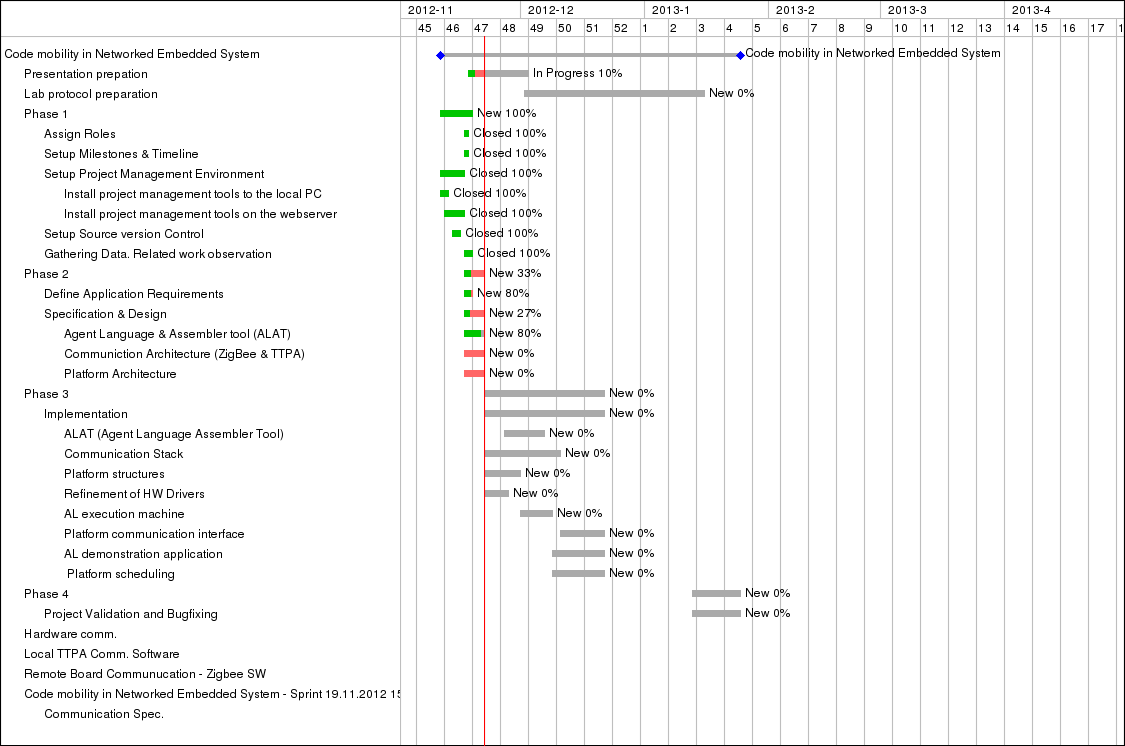
\includegraphics[scale=0.4]{figures/gantt.png}
\caption{Gantt Diagram of the Project}
\label{fig:ganttdiag}
\end{figure}


\begin{comment}
Interpreter for agent language:
\begin{itemize}
\item Agent language lexical analysis
\item Interpreter for agent language
%\item Agent language semantic analysis
\end{itemize}


Compiler for agent language:
\begin{itemize}
\item Agent language lexical analysis
\item Agent language syntax analysis
\item Agent language semantic analysis
\end{itemize}
}

Platform for mobile agents:

\begin{itemize}
\item Agent structure representation
\item Implementation of Agent structure
\item Implementation of Agent functions
\item Implementation of drivers
\item Implementation of scheduler
\item Implementation of communication protocols

\end{itemize}


%\chapter{Appendix 1}
%\chapter{Appendix 2}

%	\section{Standards}
%	\section{Training}
\end{comment}
% add other chapters and sections to suit

	\bibliography{spec}

	\bibliographystyle{plain}

\end{document}

